%%%%%%%%%%%%%%%%%%%%%%%%%%%%%%%%%%%%%%%%%%%%%%%%%%%%%%%%%%%%%%%%%%%%%%%%%%%%%%%%%%%%
% Document data
%%%%%%%%%%%%%%%%%%%%%%%%%%%%%%%%%%%%%%%%%%%%%%%%%%%%%%%%%%%%%%%%%%%%%%%%%%%%%%%%%%%%
\documentclass[12pt]{article} %report allows for chapters
%%%%%%%%%%%%%%%%%%%%%%%%%%%%%%%%%%%%%%%%%%%%%%%%%%%%%%%%%%%%%%%%%%%%%%%%%%%%%%%%%%%%
\usepackage{preamble}
\newcommand{\curvegamma}{\boldsymbol{\vec{\gamma}}}
\newcommand{\tangentgamma}{\boldsymbol{\dot{\vec{\gamma}}}}
\newcommand{\normalgamma}{\boldsymbol{\ddot{\vec{\gamma}}}}
\newcommand{\vecfieldB}{\boldsymbol{\vec{B}}}
\newcommand{\vecfieldJ}{\boldsymbol{\vec{J}}}
\newcommand{\vecfieldF}{\boldsymbol{\vec{F}}}
\newcommand{\vecx}{\boldsymbol{\vec{x}}}
\usepackage{subcaption}
\usepackage{caption}
\begin{document}

\begin{center}
   \textsc{\large MATH 272, Homework 2, \emph{Solutions}}\\
\end{center}
\vspace{.5cm}

\begin{problem}
	\textbf{(6 pts.)} Here is a plot of a 3-dimensional vector field $\vecfieldV$ when viewing from a few different angles.
	\begin{figure}[H]
		\centering
		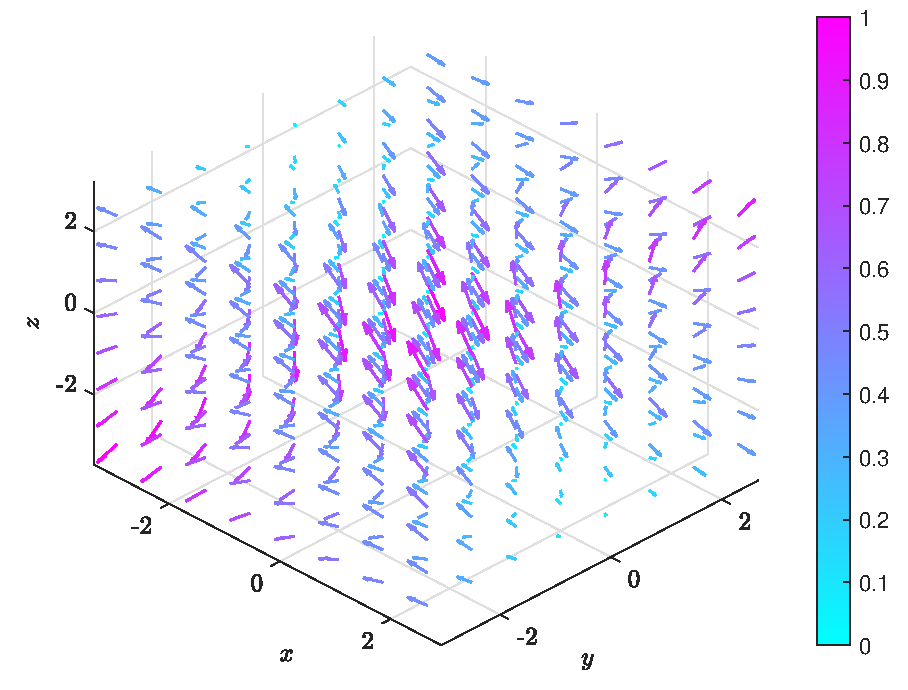
\includegraphics[width=.85\textwidth]{figures/vecfield}
		\caption{A view of the vector field $\vecfieldV$. Note that the colorscaling on this plot represents the length of the vectors. The next plots use the same colorscale.}
	\end{figure}
	\begin{figure}[H]
		\centering
		\begin{subfigure}[b]{0.45\textwidth}
			\centering
			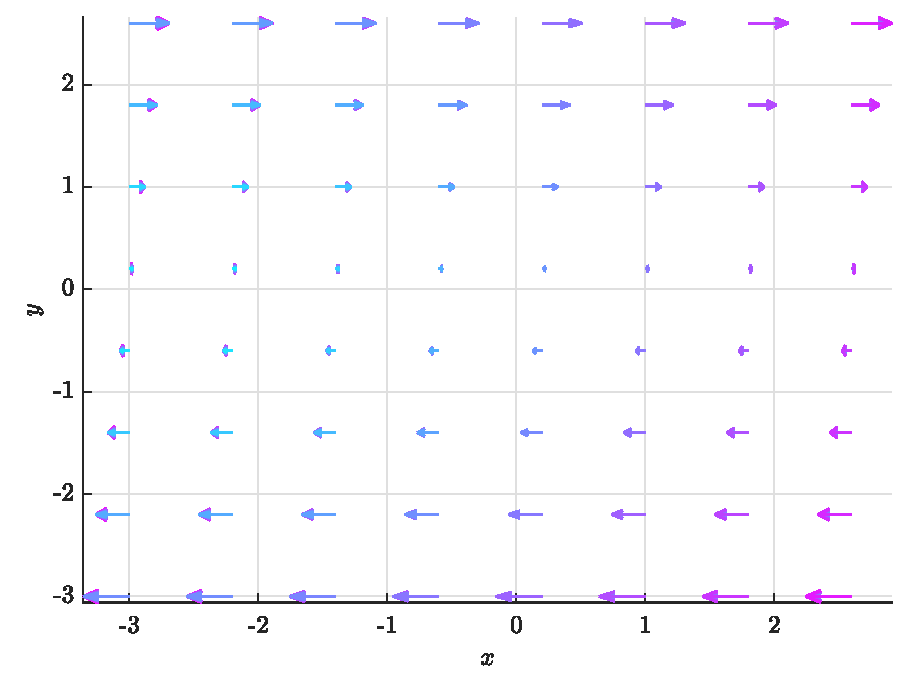
\includegraphics[width=\textwidth]{figures/vecfield_xy}
			\caption{$\vecfieldV$ when looking towards the $xy$-plane.}
		\end{subfigure}
		\quad
		\begin{subfigure}[b]{0.45\textwidth}
			\centering
			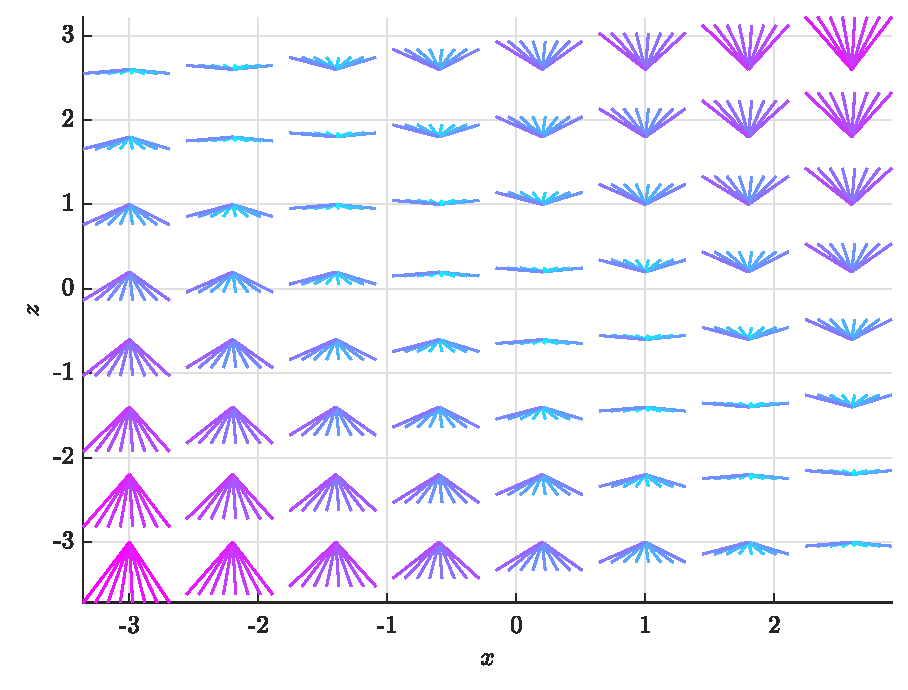
\includegraphics[width=\textwidth]{figures/vecfield_xz}
			\caption{$\vecfieldV$ when looking towards the $xz$-plane.}
		\end{subfigure}
	\end{figure}
	\begin{enumerate}[(a)]
		\item \textbf{(3 pts.)} Does this vector field have divergence? Explain.
		\item \textbf{(3 pts.)} Does this vector field have curl? Explain.
	\end{enumerate}
\end{problem}
\begin{solution}~
\begin{enumerate}[(a)]
\item Yes, let us see this by looking at the $xz$-plane image. Here, we can see that along $x=-3$, all the vectors increase their length in the $z$-direction. This would cause a particle to accelerate. One could also remark that a small circle drawn in that same region would have more outflow than inflow. This may be true in other places as well, but at the very least we can see it is true in that region.

\item Yes, take a look at the $xy$-plane image. If you placed a small rod down across the $y=0$ line, it would be pushed in opposite directions on opposite ends which causes the rod to rotate. Equivalently, a small circle parameterized in the clockwise direction placed around the $x,y=0$ in this plane would have a positive circulation or integral over that curve. So the field at least has curl if we look just off the $y=0$ line. In fact, there is curl everywhere in this plane since forces on a rod parallel to the $y$ axis would have unbalanced forces on either side.
\end{enumerate}
\end{solution}

\vspace*{1cm}
\textcolor{red}{
\noindent \textbf{Rubric:}
\begin{enumerate}[(a)]
    \item \textbf{(1 pt.)} For a correct answer. \textbf{(1 pt.)} For talking about linear acceleration of a particle or fluid flow in versus out of a circle. \textbf{(1 pt.)} For the explanation being correct.
	\item \textbf{(1 pt.)} For a correct answer. \textbf{(1 pt.)} For talking about rotation of a rod or circulation around a loop. \textbf{(1 pt.)} For the explanation being correct.
\end{enumerate}
}
\newpage

\begin{problem}
\textbf{(8 pts.)} Consider the vector field
\[
\vecfieldV(x,y,z) = \begin{pmatrix} -y \\ x \\ z \end{pmatrix}.
\]
and scalar field
\[
f(x,y,z) = x^2+y^2-z^2.
\]
\begin{enumerate}[(a)]
    \item \textbf{(2 pts.)} Compute the Jacobian (or derivative) of $\vecfieldV$.
    \item \textbf{(2 pts.)} Compute the divergence of $\vecfieldV$.
    \item \textbf{(2 pts.)} Compute the curl of $\vecfieldV$.
    \item \textbf{(2 pts.)} Compute the directional derivative of $f$ at $\vecx_0 = (1,2,-3)$ in the direction of $\vecfieldV(\vecx_0)$.
\end{enumerate}
\end{problem}
\begin{solution}
First, here is a generic view of the vector field $\vecfieldV$.
        \begin{figure}[H]
        \centering
        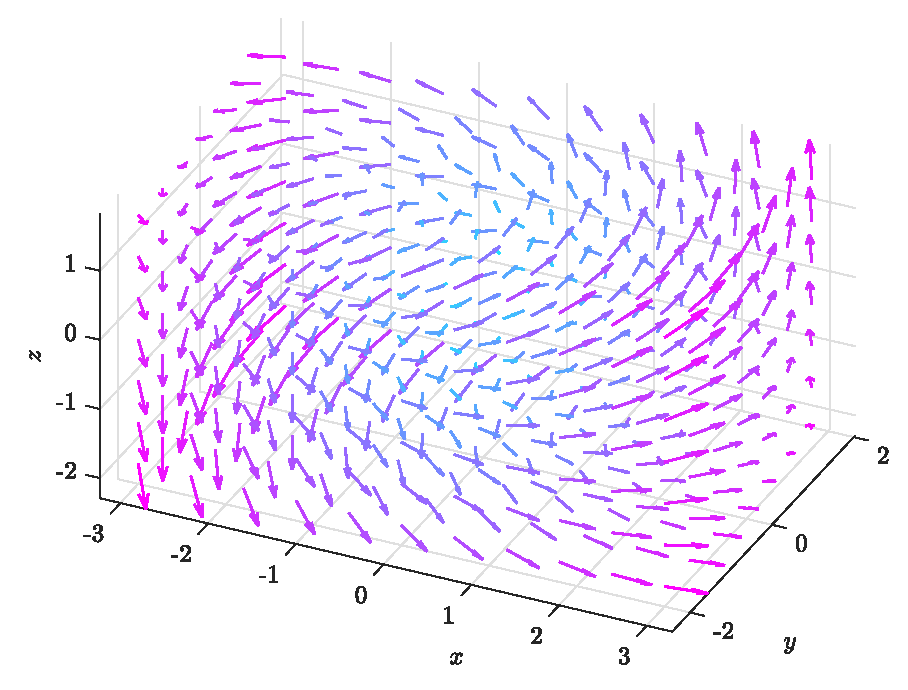
\includegraphics[width=.65\textwidth]{Figures/6c_field}
    \end{figure}
\begin{enumerate}[(a)]
	\item The derivative of the vector field $\vecfieldV$ is the matrix is written most succinctly as
	\[
	[D\vecfieldV] = \left[ \frac{\partial V_i}{\partial x_j} \right],
	\]
	where, if you'd like $x_1=x$, $x_2=y$, and $x_3=z$ (this shows you why I prefer this notation). The rows are just the gradient vectors of each of the components of $\vecfieldV$
\[
\vecfieldV = \begin{pmatrix} V_1 \\ V_2 \\ V_3 \end{pmatrix},
\]
where, of course, all of these are functions of position. We have
\begin{align*}
\grad V_1 &= \begin{pmatrix} 0 & -1 & 0 \end{pmatrix}\\
\grad V_2 &= \begin{pmatrix} 1 & 0 & 0 \end{pmatrix}\\
\grad V_3 &= \begin{pmatrix} 0 & 0 & 1 \end{pmatrix}
\end{align*}
and hence
\[
\boxed{ [D\vecfieldV]  = \begin{pmatrix} 0 & -1 & 0 \\ 1 & 0 & 0 \\ 0 & 0  & 1 \end{pmatrix}.}
\]
    \item Next, take a look at $\vecfieldV$ while aligning the $z$-axis vertically to see the following picture.
        \begin{figure}[H]
        \centering
        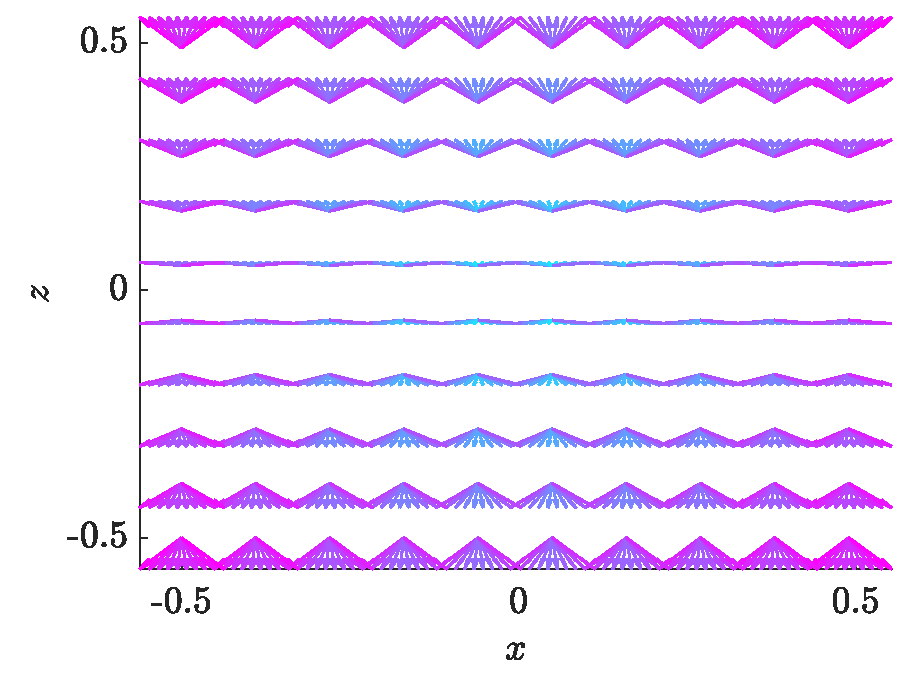
\includegraphics[width=.65\textwidth]{Figures/6d}
        \caption{Plot looking down at the $xz$-plane shows linear acceleration or source behavior.}
    \end{figure}
    If we place any particle with $z\neq 0$ then the particle will accelerate away from the $xy$-plane. Or, if we draw a circle anywhere in this plane, we can see that more fluid (arrows) will flow out of the circle than in. We expect positive divergence. To get the divergence, we have the succinct way of writing this by
\[
\grad \cdot \vecfieldV = \sum_{i=1}^3 \frac{\partial V_i}{\partial x_i} = \mathrm{tr}[D\vecfieldV] = 1.
\]
We see this explicitly using the $x,y,z,$ coordinates we may be more used to by
\[
\grad \cdot \vecfieldV = \frac{\partial V_1}{\partial x} + \frac{\partial V_2}{\partial y} + \frac{\partial V_3}{\partial z} = 0 + 0 + 1 = 1.
\]


    \item Let's examine the vector field $\vecfieldV$ by looking down at the $xy$-plane. When we do this, we see the following.
        \begin{figure}[H]
        \centering
        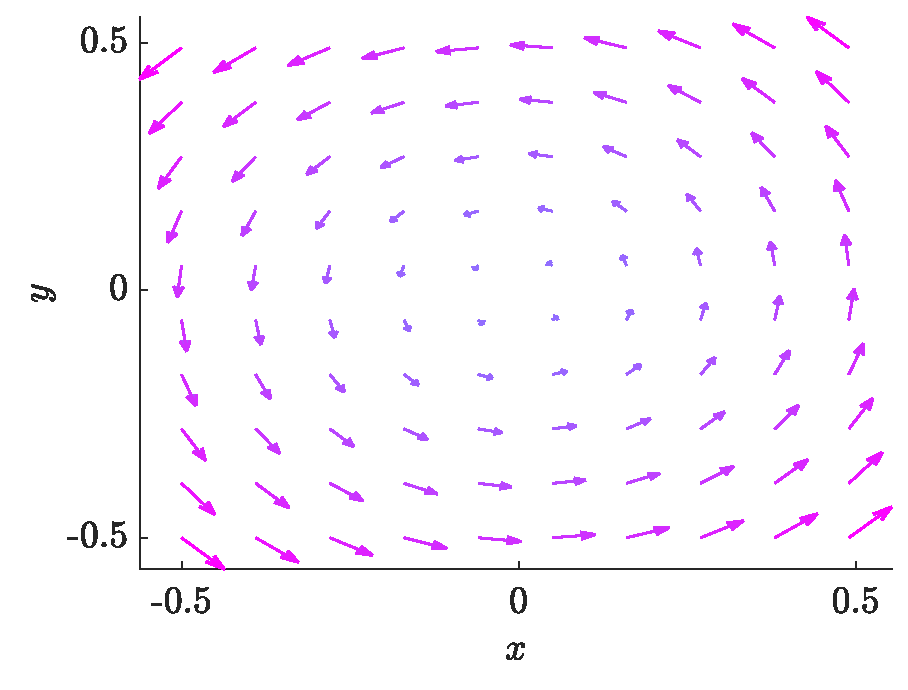
\includegraphics[width=.65\textwidth]{Figures/6c}
        \caption{Plot looking down at the $xy$-plane shows circular motion.}
    \end{figure}
    Since we see vectors that would torque a rod parallel with the $xy$-plane we that for any value of $z$ there is curl. However a particle at $x=0$ and $y=0$ will not move at all. Equivalently, the circulation around any small loop in this plane would be nonzero.

	The formula for curl is a bit convoluted, so I will avoid it here and I will use wolfram alpha to compute it. In particular I typed in 
\begin{verbatim}
curl(-y,x,z)
\end{verbatim}
and got
\begin{verbatim}
(0,0,2)
\end{verbatim}
which tells us
\[
\grad \times \vecfieldV = 2\zhat.
\]
If you would like, there is a more succinct formula for the curl as
\[
\grad \times \vecfieldV = \epsilon_{ijk} \xhat_i \frac{\partial V_j}{\partial x_k}
\]
where $\epsilon_{ijk}$ is the completely antisymmetric Levi-Civita symbol. (For more, see \url{https://en.wikipedia.org/wiki/Levi-Civita_symbol} or, if you would like, the more general way of thinking about curl begins here \url{https://en.wikipedia.org/wiki/Curl\_(mathematics)\#Generalizations}.)



    \item To compute this directional derivative, we need to compute a few items. First, we have the gradient
    \[
        \grad f = \begin{pmatrix} 2x \\ 2y \\ -2z \end{pmatrix}.
    \]
    Next, we evaluate both $\grad f$ and $\vecfieldV$ at $\vecx_0$
    \[
    \grad f(\vecx_0) = \begin{pmatrix} 2 \\ 4 \\ 6 \end{pmatrix} \qquad \textrm{and} \qquad \vecfieldV(\vecx_0) = \begin{pmatrix} -2 \\ 1 \\ -3 \end{pmatrix}.
    \]
    Now, we need a unit vector pointing in the same direction as $\vecfieldV(\vecx_0)$ so we have
    \[
    \unitvec = \frac{1}{|\vecfieldV(\vecx_0)|} \vecfieldV(\vecx_0) = \frac{1}{\sqrt{14}} \begin{pmatrix} -2 \\ 1 \\ -3 \end{pmatrix}.
    \]
    Then, the intended directional derivative is
    \[
    \boxed{\unitvec\cdot \grad f(\vecx_0) = \frac{1}{\sqrt{14}} \begin{pmatrix} -2 \\ 1 \\ -3 \end{pmatrix} \cdot \begin{pmatrix} 2 \\ 4 \\ 6 \end{pmatrix} = \frac{-18}{\sqrt{14}}.}
    \]
\end{enumerate}
\end{solution}
\vspace*{1cm}
\textcolor{red}{
\noindent \textbf{Rubric:}
\begin{enumerate}[(a)]
    \item \textbf{(1 pt.)} Correct derivatives and work (Wolfram Alpha suffices as work). \textbf{(1 pt.)} Derivatives are in the matrix in the proper way.
	\item \textbf{(1 pt.)} Correct derivatives and work (Wolfram Alpha suffices as work). \textbf{(1 pt.)} Derivatives are summed up in the proper way and, for example, \textbf{not} put into a vector.
	\item \textbf{(1 pt.)} Correct derivatives and work (Wolfram Alpha suffices as work) \textbf{(1 pt.)} Derivatives are put together properly and the output is a vector.
	\item \textbf{(1 pt.)} Correct derivatives and work (Wolfram Alpha suffices as work) \textbf{(1 pt.)} Output is a the correct number and not a vector and no variables are left; This means all the variables had to be properly plugged in.
\end{enumerate}
}


\newpage

\begin{problem}
\textbf{(8 pts.)} Consider the following vector field
\[
\vecfieldB = -\frac{y}{2}\xhat + \frac{x}{2}\yhat.
\]
Here, $\vecfieldB$ denotes the magnetic field. It may be helpful to plot the fields in this problem.
\begin{enumerate}[(a)]
    \item \textbf{(1 pts.)} Show that $\vecfieldB$ has no divergence. (This is one of Gauss's laws.)
    \item \textbf{(1 pts.)} Show that $\grad \times \vecfieldB = \vecfieldJ$ (Amp\'ere's law) where
    \[
    \vecfieldJ = \zhat.
    \]
    This vector field $\vecfieldJ$ represents the electric current (moving charges) in space. One could argue that the current creates the magnetic field via Amp\'ere's law.
    \item \textbf{(4 pts.)} Magnetic fields induce a force $\vecfieldF$ on charged particles by the Lorentz force
    \[
    \vecfieldF = \tangentgamma \times \vecfieldB = \normalgamma
    \]
    Where $\tangentgamma$ is the velocity of the particle (where we have chosen a mass $m=1$ and charge $q=1$).  Let us do the following.
    \begin{itemize}
        \item Assume that $\tangentgamma = \xhat$, what is the force on the particle?
        \item Repeat the previous step for $\tangentgamma=\yhat$ and $\tangentgamma=\zhat$.
        \item Compare and contrast the forces you found.
    \end{itemize}
    \item \textbf{(2 pts.)} Can you argue why applying a magnetic field to a molecule may cause it to heat up? Can you compare this idea with your home microwave?
\end{enumerate}
\end{problem}
\begin{solution}~
\begin{enumerate}[(a)]
	\item We have
\[
\grad \cdot \vecfieldB = \frac{\partial}{\partial x} \left(\frac{-y}{2}\right) + \frac{\partial}{\partial y} \left(\frac{x}{2} \right) = 0.
\]
    \item We have
    \begin{align*}
        \begin{pmatrix} \frac{\partial}{\partial x} \\ \frac{\partial}{\partial y} \\ \frac{\partial}{\partial z} \end{pmatrix} \times \begin{pmatrix} \frac{-y}{2} \\ \frac{x}{2} \\ 0 \end{pmatrix} &= \begin{pmatrix} 0 \\ 0 \\   \frac{\partial}{\partial x} \frac{x}{2} - \frac{\partial}{\partial y} \frac{-y}{2} \end{pmatrix} \\
                &= \begin{pmatrix} 0 \\ 0 \\ 1 \end{pmatrix}\\
                &= \zhat.
    \end{align*}
    \item We will look at the case for the three different tangent vectors.
    \begin{itemize}
        \item If $\tangentgamma = \xhat$, then
        \[
        \tangentgamma \times \vecfieldB = \frac{x}{2}\zhat.
        \]
        \item If $\tangentgamma = \yhat$, then
        \[
        \tangentgamma \times \vecfieldB = \frac{y}{2} \zhat.
        \]
        \item Finally, if $\tangentgamma =\zhat$, then
        \[
        \tangentgamma \times \vecfieldB = -\frac{y}{2}\yhat -\frac{x}{2}\xhat.
        \]
    \end{itemize}
    Note that if $\tangentgamma$ is in the $x$- or $y$-direction, we get a force that is aligned in the $z$-direction. Moreover, in those cases the forces will cause the particle to accelerate away indefinitely in the $z$-direction. That is, so long as the $x\neq 0$ in the first case and $y\neq 0$ in the second.

	In the last case, when $\tangentgamma$ is in the $z$-direction, then the forces are in the $x$- and $y$-direction. This means the particle will continue to move in the $z$-direction at constant velocity, but the particle will oscillate over the $xy$-plane since the forces are equal and opposite to the $x$ and $y$ component of the curve $\curvegamma$. In fact, this actually looks like Hooke's law.

    \item If we apply a magnetic field to charged particles, the particles can experience nonzero forces. By applying forces, the particles receive more energy of motion and this means that we are heating them up.  If we apply the correct kind of magnetic field, it is conceivable that we would simply causes a particle to vibrate with more intensity. The vibration would come in the case of our last example in part (c). Microwaves work by applying fairly strong magnetic fields to your food. The charge imbalance in $H_2 O$ leads to water molecules absorbing energy from this field.
\end{enumerate}
\end{solution}
\vspace*{1cm}
\textcolor{red}{
\noindent \textbf{Rubric:}
\begin{enumerate}[(a)]
    \item \textbf{(1 pt.)} Correct answer and work.
	\item \textbf{(1 pt.)} Correct answer and work.
	\item \textbf{(3 pt.)} Correct answer and work for each of the different tangent vectors $\tangentgamma$. \textbf{(1 pt.)} For comparing and contrasting properly.
	\item \textbf{(1 pt.)} Reasonable explanation for how this can give energy to charges. \textbf{(1 pt.)} A good explanation for what a microwave does. 
\end{enumerate}
}

\newpage

\begin{problem}
\textbf{(6 pts.)} Consider the function
\[
f(x,y)=\sin\left(\frac{2\pi x}{5}\right)\sin\left(\frac{2\pi y}{5}\right).
\]
comes up when you want to find out how a square shaped drum head will vibrate when hit.
\begin{enumerate}[(a)]
    \item \textbf{(1 pts.)} Plot this function on the region $\Omega$ given by $0\leq x \leq 5$ and $0\leq y \leq 5$.
    \item \textbf{(2 pts.)} What is the value the function $f(x,y)$ on the boundary of the given region $\Omega$ (i.e, when $x=0$, $x=5$, $y=0$, and $y=5$)?
    \item \textbf{(3 pts.)} Show that $f(x,y)$ is an eigenfunction of the Laplacian $\Delta$. That is, $\Delta f = \lambda f$ for some eigenvalue $\lambda$. What is the eigenvalue?
\end{enumerate}
\end{problem}
\begin{solution}~
\begin{enumerate}[(a)]
    \item Here is the plot of the vibrating square drum head:
    \begin{figure}[H]
        \centering
	\def\svgwidth{0.75\columnwidth}
	\input{Figures/drum_head.pdf_tex}
    \end{figure}
    \item When $x=0$ we have
    \[
    f(0,y) = \sin\left( \frac{2\pi 0}{5}\right) \sin\left(\frac{2\pi y}{5}\right) = 0.
    \]
    Similarly, when $x=5$ $f(5,y)=0$, when $y=0$ $f(x,0)=0$, and when $y=5$ $f(x,5)=0$.

    These are the boundary of the drum head.  That is, where the head of the drum is clamped down.

    \item We have
    \begin{align*}
        \frac{\partial f}{\partial x} &= \frac{2\pi}{5} \cos \left( \frac{2\pi x}{5} \right) \sin \left( \frac{2\pi y}{5} \right),\\
        \frac{\partial^2 f}{\partial x^2} &= \frac{-4\pi^2}{25} \sin \left( \frac{2\pi x}{5} \right) \sin \left( \frac{2\pi y}{5} \right),\\
        \frac{\partial f}{\partial y} &= \frac{2\pi}{5} \sin \left( \frac{2\pi x}{5} \right) \cos \left( \frac{2\pi y}{5} \right),\\
        \frac{\partial^2 f}{\partial y^2} &= \frac{-4\pi}{25} \sin \left( \frac{2\pi x}{5} \right) \sin \left( \frac{2\pi y}{5} \right).
    \end{align*}
    Then we have
    \[
    \frac{\partial^2 f}{\partial x^2} + \frac{\partial^2 f}{\partial y^2} = -\frac{8\pi^2}{25} \sin \left( \frac{2\pi x}{5} \right) \sin \left( \frac{2\pi y}{5} \right) = -\frac{8\pi^2}{25} f(x,y).
    \]
    So, the way a drum head vibrates is an eigen-problem.
\end{enumerate}
\end{solution}
\vspace*{1cm}
\textcolor{red}{
\noindent \textbf{Rubric:}
\begin{enumerate}[(a)]
    \item \textbf{(1 pt.)} Correct plot with correct bounds.
    \item \textbf{(2 pt.)} Correct work by plugging in \textbf{all of} the relevant values of $x$ and $y$. 
    \item \textbf{(1 pt.)} Correct second partials. \textbf{(1 pt.)} Laplacian is a scalar $\lambda$ times the original function but potentially not simplified. \textbf{(1 pt.)} Explains what the value for $\lambda$ is.
\end{enumerate}
}

\newpage

\begin{problem}
\textbf{(12 pts.)} For the following, describe the composite function as a function $\R^m \to \R^n$, in other words, what is the dimension of the domain and codomain? Then, compute the composite function given to you and write down if there are any other possible composite functions you could make. Finally, what are the dimensions of the matrix that correspond to the derivative of the composite function?
\begin{enumerate}[(a)]
\item \textbf{(4 pts.)} Take $f\colon \R^2 \to \R$ given by $f(x,y)=\sin(xy)$ and let $\curvegamma \colon \R \to \R^2$ be given by $\curvegamma(t) = \begin{pmatrix} t \\ 1 \end{pmatrix}$. The composite function $f\circ \curvegamma$.
\item \textbf{(4 pts.)} Take $\vecfieldV \colon \R^2 \to \R^2$ by $\vecfieldV(x,y)= \begin{pmatrix} xy \\ x+y \end{pmatrix}$ and let $\curvegamma \colon \R \to \R^2$ by $\curvegamma(t) = \begin{pmatrix} \cos(t) \\ \cos^2(t) \end{pmatrix}$. The composite function $\vecfieldV \circ \curvegamma$.
\item \textbf{(4 pts.)} Take $\vecfieldV \colon \R^3 \to \R^3$ by $\vecfieldV(x,y)= \begin{pmatrix} xz \\ yz \\ z^2 \end{pmatrix}$ and let $f \colon \R^3 \to \R$ by $f(x,y,z) = xz + yz + z^2$. The composite function $f\circ \vecfieldV$.
\end{enumerate}
\end{problem}
\begin{solution}~
\begin{enumerate}[(a)]
	\item We have that
	\[
	f\circ \curvegamma \colon \R \to \R.
	\]
	Specifically,
	\[
	\boxed{f(\curvegamma(t)) = \sin(t).}
	\]
	The shape of the matrix for the derivative of this composite function would be $1\times 1$ since both the input and output are 1-dimensional.

	We could also compute
	\[
	\curvegamma \circ f \colon \R^2 \to \R^2
	\]
	in this case.

	\item We have that
	\[
	\vecfieldV \circ \curvegamma \colon \R \to \R^2.
	\]
	Specifically,
	\[
	\boxed{\vecfieldV(\curvegamma(t)) = \begin{pmatrix} \cos^3(t) \\ \cos(t) + \cos^2(t) \end{pmatrix}.}
	\]
	The shape of the matrix for the derivative of this composite function would be $2\times 1$ since both the output is 2-dimensional and the input is 1-dimensional. 

	There are no other composite functions to compute since $\curvegamma \circ \vecfieldV$ cannot possibly work.

	\item We have that
	\[
	f\circ \vecfieldV \colon \R^3 \to \R.
	\]
	Specifically,
	\[
	\boxed{f(\vecfieldV(x,y,z)) = (xz)(z^2)+(yz)(z^2)+(z^2)^2.}
	\]
	The shape of the matrix for the derivative of this composite function would be $1\times 3$ since the input is 3-dimensional and the output is 1-dimensional.

	There are no other composite functions to compute since $\vecfieldV \circ f$ cannot possibly work.
\end{enumerate}
\end{solution}
\vspace*{1cm}
\textcolor{red}{
\noindent \textbf{Rubric:}
\begin{enumerate}[(a)]
    \item \textbf{(1 pt.)} Correct input and output dimension for composite. \textbf{(1 pt.)} Correct composite function. \textbf{(1 pt.)} Correct dimensions of derivative matrix. \textbf{(1 pt.)} Correct answer for other possible composite function.
	\item \textbf{(1 pt.)} Correct input and output dimension for composite. \textbf{(1 pt.)} Correct composite function. \textbf{(1 pt.)} Correct dimensions of derivative matrix. \textbf{(1 pt.)} Correct answer for other possible composite function.
	\item \textbf{(1 pt.)} Correct input and output dimension for composite. \textbf{(1 pt.)} Correct composite function. \textbf{(1 pt.)} Correct dimensions of derivative matrix. \textbf{(1 pt.)} Correct answer for other possible composite function.
\end{enumerate}
}
\newpage

\begin{problem}
\textbf{(12 pts.)} Set up but do not compute the integrals of the given fields over the given curves.
    \begin{enumerate}[(a)]
        \item \textbf{(3 pts.)} $f(x,y) = xe^{x+y}+\cos(xy)$, $\curvegamma(t) = \begin{pmatrix} \cos(t) \\ \sin(t) \end{pmatrix}$, $t_0 = 0$, $t_1=2\pi$.
        \item \textbf{(3 pts.)} $g(x,y,z) = \frac{\ln(z^2)}{e^{xy}}$, $\curvegamma(t) = \begin{pmatrix} t \\ t^2 \\ t^3 \end{pmatrix}$ , $t_0 = 1$, $t_1=-1$.
        \item \textbf{(3 pts.)} $\vecfieldU(x,y) = \begin{pmatrix} -y \\ x \end{pmatrix}$, $\curvegamma(t) = \begin{pmatrix} e^t \\ e^t \end{pmatrix}$, $t_0 = 5$, $t_1=10$.
        \item \textbf{(3 pts.)} $\vecfieldV(x,y,z) = \begin{pmatrix} 2x \\ y \\ x \end{pmatrix}$, $\curvegamma(t) = \begin{pmatrix} \cos(t) \\ t \\ \sqrt{t} \end{pmatrix}$, $t_0 = 0$, $t_1=1$.
    \end{enumerate}
\end{problem}
\begin{solution}~
\begin{enumerate}[(a)]
    \item We want to integrate
    \[
    \int_{\curvegamma} f d\curvegamma = \int_{t_0}^{t_1} f(\curvegamma(t)) \left| \tangentgamma(t) \right| dt.
    \]
    We just have to determine each part of this integral. We know $t_0$ and $t_1$, so we just need $f(\curvegamma(t))$ and the speed $\left|\tangentgamma(t)\right|$. Evaluating yields,
    \[
    f(\curvegamma(t)) = \cos(t)e^{\cos(t)+\sin(t)} + \cos(\cos(t)\sin(t)),
    \]
    and
    \[
    \tangentgamma(t) = \begin{pmatrix} -\sin(t) \\ \cos(t) \end{pmatrix}
    \]
    which means
    \[
    \left| \tangentgamma(t) \right| = \sqrt{\sin^2(t) + \cos^2(t)} = 1.
    \]
    Thus, we have
    \[
    \boxed{\int_{\curvegamma} f d\curvegamma = \int_0^{2\pi} \cos(t)e^{\cos(t)+\sin(t)} + \cos(\cos(t)\sin(t)) dt.}
    \]

    \item This part is analogous to (a), so we have
    \[
    g(\curvegamma(t)) = \frac{\ln(t^6)}{e^{t^3}},
    \]
    \[
    \tangentgamma(t) = \begin{pmatrix} 1 \\ 2t \\ 3t^2 \end{pmatrix},
    \]
    therefore
    \[
    \left| \tangentgamma(t) \right| = \sqrt{1+4t^2+9t^4}.
    \]
    Thus,
    \[
    \boxed{\int_{\curvegamma} g d\curvegamma = \int_{1}^{-1} \frac{\ln(t^6)}{e^{t^3}} \sqrt{1+4t^2+9t^4} dt.}
    \]

    \item We want to integrate
    \[
    \int_{\curvegamma} \vecfieldU \cdot d\curvegamma = \int_{t_0}^{t_1} \vecfieldU(\curvegamma(t)) \cdot \tangentgamma(t) dt.
    \]
    So, we determine each individual part of this integral. We have
    \[
    \vecfieldU(\curvegamma(t)) = \begin{pmatrix} -e^t \\ e^t \end{pmatrix}
    \]
    and
    \[
    \tangentgamma(t) = \begin{pmatrix} e^t \\ e^t \end{pmatrix}.
    \]
    Lastly, we compute the dot product
    \[
    \vecfieldU(\curvegamma(t)) \cdot \tangentgamma(t) = -e^{2t} + e^{2t} = 0.
    \]
    Thus,
    \[
    \boxed{\int_{\curvegamma} \vecfieldU \cdot d\curvegamma = \int_{5}^{10} 0 dt = 0.}
    \]

    \item This part is analogous to (c). We have
    \[
    \vecfieldV(\curvegamma(t)) = \begin{pmatrix} 2 \cos(t) \\ t \\ \cos(t) \end{pmatrix}
    \]
    and
    \[
    \tangentgamma(t) = \begin{pmatrix} -\sin(t) \\ 1 \\ \frac{1}{2\sqrt{t}} \end{pmatrix}.
    \]
    Then,
    \[
    \vecfieldV(\curvegamma(t)) \cdot \tangentgamma(t) = -2 \cos(t) \sin(t) + t + \frac{\cos(t)}{2\sqrt{t}}.
    \]
    Thus,
    \[
    \boxed{\int_{\curvegamma} \vecfieldV \cdot d\curvegamma = \int_0^1 -2 \cos(t) \sin(t) + t + \frac{\cos(t)}{2\sqrt{t}} dt.}
    \]
\end{enumerate}
\end{solution}
\vspace*{1cm}
\textcolor{red}{
\noindent \textbf{Rubric:}
\begin{enumerate}[(a)]
    \item \textbf{(1 pt.)} Correct composite function. \textbf{(1 pt.)} Correct speed $|\tangentgamma|$. \textbf{(1 pt.)} Integrand and bounds are set correctly.
    \item \textbf{(1 pt.)} Correct composite function. \textbf{(1 pt.)} Correct speed $|\tangentgamma|$. \textbf{(1 pt.)} Integrand and bounds are set correctly.
    \item \textbf{(1 pt.)} Correct composite function. \textbf{(1 pt.)} Correct velocity $\tangentgamma$. \textbf{(1 pt.)} Integrand and bounds are set correctly and dot product with velocity is taken.
    \item \textbf{(1 pt.)} Correct composite function. \textbf{(1 pt.)} Correct velocity $\tangentgamma$. \textbf{(1 pt.)} Integrand and bounds are set correctly and dot product with velocity is taken.
\end{enumerate}
}

\newpage
\begin{problem}
\textbf{(4 pts.)} Let $f(x,y,z)=x \cos(y) + yz$ be a scalar field and let $\curvegamma = \begin{pmatrix} 1 \\ t \\ \sin(t) \end{pmatrix}$ be a curve from time $t_0 = 0$ to $t_1 = 2 \pi$. Compute
\[
    \int_{\curvegamma} f(\curvegamma)d\curvegamma.
\]
\end{problem}
\begin{solution}
First,
\[
f(\curvegamma(t)) = \cos(t) + t \sin(t),
\]
\[
\tangentgamma(t) = \begin{pmatrix} 0 \\ 1 \\ \cos(t) \end{pmatrix},
\]
and
\[
\left| \tangentgamma(t) \right| = \sqrt{1+\cos^2(t)}.
\]
Thus, we now compute
\begin{align*}
    \int_{\curvegamma} f(\curvegamma)d\curvegamma & = \int_0^{2\pi} (\cos(t) + t \sin(t)) \sqrt{1+\cos^2(t)} dt\\
    &\approx -7.2118.
\end{align*}
This was computed using WolframAlpha by inputting:
\begin{verbatim}
integrate[(cos(t)+t sin(t)) sqrt(1+cos^2(t)), {t,0,2pi}]
\end{verbatim}
\end{solution}
\vspace*{1cm}
\textcolor{red}{
\noindent \textbf{Rubric:}
\begin{enumerate}[(a)]
    \item \textbf{(1 pt.)} Correct composite function and correct speed $|\tangentgamma|$. \textbf{(1 pt.)} Integrand and bounds are set correctly. \textbf{(2 pts.)} Correct value for integral.
\end{enumerate}
}

\newpage
\begin{problem}
\textbf{(4 pts.)} Show that for any smooth (more than twice differentiable) fields $f(x,y,z)$ and $\vecfieldV(x,y,z)$ that
\begin{enumerate}[(a)]
	\item \textbf{(2 pts.)} $\grad \times \left(\grad f\right)=\boldsymbol{\vec{0}}$;
	\item \textbf{(2 pts.)} $\grad \cdot \left(\grad \times \vecfieldV\right)=0$.
\end{enumerate}
\end{problem}
\begin{solution}~
    \begin{enumerate}[(a)]
        \item We have that 
        \[
        \grad f = \begin{pmatrix} \frac{\partial f}{\partial x} \\ \frac{\partial f}{\partial y} \\ \frac{\partial f}{\partial z}\end{pmatrix} = \begin{pmatrix} V_1 \\ V_2 \\ V_3 \end{pmatrix}.
        \]
        Taking the curl yields
        \[
        \grad \times \left(\grad f\right) = \begin{pmatrix} \frac{\partial V_3}{\partial y} - \frac{\partial V_2}{\partial z} \\ \frac{\partial V_1}{\partial z} - \frac{\partial V_3}{\partial x} \\ \frac{\partial V_2}{\partial x} - \frac{\partial V_1}{\partial y} \end{pmatrix} = 
        \begin{pmatrix} \frac{\partial^2 f}{\partial z\partial y} - \frac{\partial^2 f}{\partial y\partial z} \\ \frac{\partial^2 f}{\partial x\partial z} - \frac{\partial^2 f}{\partial z \partial x} \\ \frac{\partial^2 f}{\partial y\partial x} - \frac{\partial f}{\partial x\partial y} \end{pmatrix}= \begin{pmatrix} 0 \\ 0 \\ 0 \end{pmatrix},
        \]
        since partial derivatives commute for any smooth scalar field.
        
        \item First, the curl is
        \[
        \grad \times \vecfieldV = \begin{pmatrix} \frac{\partial V_3}{\partial y} - \frac{\partial V_2}{\partial z} \\ \frac{\partial V_1}{\partial z} - \frac{\partial V_3}{\partial x} \\ \frac{\partial V_2}{\partial x} - \frac{\partial V_1}{\partial y} \end{pmatrix},
        \]
        and we can take the divergence
        \begin{align*}
            \grad \cdot \left(\grad \times \vecfieldV\right) &= \frac{\partial}{\partial x} \left(\frac{\partial V_3}{\partial y} - \frac{\partial V_2}{\partial z}\right) +  \frac{\partial}{\partial y} \left(\frac{\partial V_1}{\partial z} - \frac{\partial V_3}{\partial x}\right) +  \frac{\partial}{\partial z} \left(\frac{\partial V_2}{\partial x} - \frac{\partial V_1}{\partial y}\right)\\
            &= 0,
        \end{align*}
        again since partial derivatives commute.
    \end{enumerate}
\end{solution}
\vspace*{1cm}
\textcolor{red}{
\noindent \textbf{Rubric:}
\begin{enumerate}[(a)]
    \item \textbf{(1 pt.)} Applying the derivatives to a \textbf{arbitrary field $f$} not some specifically chosen function! \textbf{(1 pt.)} Correct work.
    \item \textbf{(1 pt.)} Applying the derivatives to a \textbf{arbitrary field $\vecfieldV$} not some specifically chosen function! \textbf{(1 pt.)} Correct work.
\end{enumerate}
}

\newpage
\begin{problem}
\textbf{(5 pts.)} Let
	\[
	\vecfieldU(x,y,z) = \begin{pmatrix} -y \\ x \\ 0 \end{pmatrix} \qquad \textrm{and} \qquad \vecfieldV(x,y,z) = \begin{pmatrix} 2x \\ 2y \\ 2z \end{pmatrix},
	\]
	be vector fields.
	\begin{enumerate}[(a)]
		\item \textbf{(1 pts.)} Explain why there exists no potential function $\phi(x,y,z)$ for the vector field $\vecfieldU$.
		\item \textbf{(1 pts.)} Explain why there does exist a potential function $\phi(x,y,z)$ for the field $\vecfieldV$.
		\item \textbf{(3 pts.)} Compute the potential function for $\vecfieldV$.
	\end{enumerate}
\end{problem}
\begin{solution}~
    \begin{enumerate}[(a)]
        \item There exists a potential function if the curl of $\vecfieldU$ is zero.  So, taking the curl we find
        \[
        \grad \times \vecfieldU = \begin{pmatrix} 0 \\ 0 \\ 2 \end{pmatrix},
        \]
        which is nonzero. Thus, there cannot be a potential function for $\vecfieldU$.
        
        \item Likewise, taking the curl for $\vecfieldV$ we get
        \[
            \grad\times \vecfieldU = \begin{pmatrix} 0 \\ 0 \\ 0 \end{pmatrix}.
        \]
        Hence, there must be a potential function for $\vecfieldV$.  
        
        \item To compute the potential $\phi(x,y,z)$, we integrate $V_1$ with respect to $x$, $V_2$ with respect to $y$, and $V_3$ with respect to $z$.  This yields
        \begin{align*}
            \phi(x,y,z) &= \int 2x dx = x^2+\psi_1(y,z)\\
            \phi(x,y,z) &= \int 2y dy = y^2+\psi_2(x,z)\\
            \phi(x,y,z) &= \int 2z dz = z^2+\psi_3(x,y).
        \end{align*}
        Since these are all equal, we must have that
        \[
        \boxed{\phi(x,y,z) = x^2+y^2+z^2+C,}
        \]
        where $C$ is a constant.
    \end{enumerate}
\end{solution}
\vspace*{1cm}
\textcolor{red}{
\noindent \textbf{Rubric:}
\begin{enumerate}[(a)]
    \item \textbf{(1 pt.)} Show that $\grad \times \vecfieldU \neq \zerovec$.
	\item \textbf{(1 pt.)} Show that $\grad \times \vecfieldV = \zerovec$.
	\item \textbf{(2 pt.)} Integrate the components of $\vecfieldV$ with respect to the correct variables. \textbf{(1 pt.)} Identify that there are the functions $\psi_i$ and determine the potential $\phi$ up to a constant.
\end{enumerate}
}

\newpage
\begin{problem}
\textbf{(10 pts.)} Consider the following vector field
    \[
    \vecfieldE = \frac{x}{\left(x^2+y^2+z^2\right)^{3/2}} \xhat + \frac{y}{\left(x^2+y^2+z^2\right)^{3/2}} \yhat + \frac{z}{\left(x^2+y^2+z^2\right)^{3/2}} \zhat,
    \]
    which you can think of as the electric field of a positive point charge.  It turns out that this field $\vecfieldE$ is conservative (which you will show in (a)). Specifically, $\vecfieldE = -\grad \phi$, for the scalar field
\[
\phi(x,y,z) = \frac{1}{\sqrt{x^2+y^2+z^2}}
\]
This is Faraday's law for static fields.
    \begin{enumerate}[(a)]
        \item \textbf{(2 pts.)} Compute the divergence and curl of $\vecfieldE$. What can we say about the vector field, its divergence, and its curl at the origin?
        \item \textbf{(3 pts.)} Compute the integral
        \[
        T=\int_{\curvegamma} \vecfieldE \cdot d\curvegamma \qquad \textrm{where} \qquad \curvegamma(t) = \begin{pmatrix} t \\ t \\ t \end{pmatrix},
        \]
        and $t\in [t_0,t_1]$ with $t_0$ and $t_1$ both greater than 0.  Note that this integral $T$ describes the gain in kinetic energy of a charged particle that moved along the path $\curvegamma$.
        \item \textbf{(3 pts.)} Equivalently, since $\vecfieldE$ is conservative, we have
        \[
        T=\int_{\curvegamma} \vecfieldE \cdot d\curvegamma = \phi(\curvegamma(t_1))-\phi(\curvegamma(t_0)).
        \]
        Show that this is true for the given vector field and potential. This shows that the choice of path does not matter; only the endpoints $\curvegamma(t_0)$ and $\curvegamma(t_1)$ matter.
        \item \textbf{(2 pts.)} Argue why the integral around any closed curve must be zero.
    \end{enumerate}
\end{problem}
\begin{solution}~
\begin{enumerate}[(a)]
   	\item First, let us take the curl of $\vecfieldE$.  We have
    \begin{align*}
        \grad \times \vecfieldE &= \begin{pmatrix} \frac{\partial E_3}{\partial y} - \frac{\partial E_2}{\partial z} \\ \frac{\partial E_1}{\partial z} -\frac{\partial E_3}{\partial 1} \\ \frac{\partial E_2}{\partial x} - \frac{\partial E_1}{\partial y} \end{pmatrix}\\
        &= \begin{pmatrix} \frac{-3yz}{(x^2+y^2+z^2)^{5/2}} - \frac{-3yz}{(x^2+y^2+z^2)^{5/2}} \\ \frac{-3xz}{(x^2+y^2+z^2)^{5/2}} - \frac{-3xz}{(x^2+y^2+z^2)^{5/2}} \\
        \frac{-3xy}{(x^2+y^2+z^2)^{5/2}} -\frac{-3xy}{(x^2+y^2+z^2)^{5/2}} \end{pmatrix}\\
        &= \begin{pmatrix} 0 \\ 0 \\ 0 \end{pmatrix}.
    \end{align*}
    At the origin, this curl is also identically zero.  The curl of $\vecfieldE$ is simply zero everywhere. One can also just use the fact from Problem 8 in that we know that $\grad \times (\grad f) = 0$ and since $\vecfieldE = -\grad \phi$ we know $\grad \times \vecfieldE = -\grad \times (\grad \phi) = 0$.

    The divergence of $\vecfieldE$ is
    \begin{align*}
        \grad \cdot \vecfieldE &= \frac{\partial E_1}{\partial x} + \frac{\partial E_2}{\partial y} + \frac{\partial E_3}{\partial z}\\
        &= \frac{-2x^2+y^2+z^2}{(x^2+y^2+z^2)^{5/2}} + \frac{x^2-2y^2+z^2}{(x^2+y^2+z^2)^{5/2}} + \frac{x^2+y^2-2z^2}{(x^2+y^2+z^2)^{5/2}}\\
        &= 0.
    \end{align*}
    It appears that the divergence of this field $\vecfieldE$ is zero, however this is not actually true at the origin. We will revisit this later, but for now it should be fairly clear that the denominator goes to zero more quickly than the numerator. Indeed, we actually have
    \[
        \grad \cdot \vecfieldE = \delta(\vecx),
    \]
    where $\delta(\vecx)$ is the Dirac delta mass (i.e., a point charge/mass).


    \item First, note that
    \[
    d\curvegamma = \tangentgamma(t) dt = (\xhat + \yhat + \zhat)dt.
    \]
    Thus, we have that
    \[
    \vecfieldE(\curvegamma(t))= \frac{t}{\left(3t^2\right)^{3/2}} \xhat + \frac{t}{\left(3t^2\right)^{3/2}} \yhat + \frac{t}{\left(3t^2\right)^{3/2}} \zhat,
    \]
    and therefore
    \[
    \vecfieldE(\curvegamma(t)) \cdot d\curvegamma = \frac{3t}{\left(3t^2\right)^{3/2}}dt = \frac{1}{t^2\sqrt{3}}dt.
    \]
    Now, we have
    \begin{align*}
        \int_{\curvegamma} \vecfieldE \cdot d\gamma &= \int_{t_0}^{t_1} \frac{1}{t^2\sqrt{3}}dt\\
        &= \frac{-1}{\sqrt{3}}\left(\frac{1}{t_1} - \frac{1}{t_0}\right).
    \end{align*}
    \item Note that we have
    \[
    \phi(x,y,z) = \frac{-1}{\sqrt{x^2+y^2+z^2}},
    \]
    and we can evalute
    \begin{align*}
        \phi(\curvegamma(t_1))-\phi(\curvegamma(t_0)) &= \frac{-1}{\sqrt{3t_1^2}}-\frac{1}{\sqrt{3t_0^2}}\\
        &= \frac{-1}{\sqrt{3}} \left(\frac{1}{t_1}-\frac{1}{t_0}\right),
    \end{align*}
    which is identical to the answer from (a).
    \item For a closed curve, we have $\curvegamma(t_1)=\curvegamma(t_0)$ and thus
    \[
    \int_{\curvegamma} \vecfieldE \cdot d\gamma = \phi(\curvegamma(t_1))-\phi(\curvegamma(t_0)) = \phi(\curvegamma(t_0))-\phi(\curvegamma(t_0))=0.
    \]
\end{enumerate}
\end{solution}
\vspace*{1cm}
\textcolor{red}{
\noindent \textbf{Rubric:}
\begin{enumerate}[(a)]
    \item \textbf{(1 pt.)} Correct divergence and curl. \textbf{Give a bonus point if Problem 8 is used for the curl argument.} \textbf{(1 pt.)} A mention of what happens at the origin.
	\item \textbf{(2 pt.)} Correct integrand and bounds for integral set up. \textbf{(1 pt.)} Correct value for the integral with the arbitrary $t_0$ and $t_1$.
	\item \textbf{(2 pt.)} Correct composite function and showing that the answer is that of (b) (note that I actually typoed and forgot the minus sign $\vecfieldE= -\grad \phi$ so if this causes sign issues, don't mark off for that). \textbf{(1 pt.)} Argument on why this shows that path does not matter.
	\item \textbf{(2 pt.)} Correct argument saying that the endpoints are the same so we get zero using the equation in (c).
\end{enumerate}
}

\newpage
\begin{problem}
\textbf{(3 pts.)} Let $f(x,y,z)=2xy+e^{xz}+\sin(y)$ be a scalar field. Integrate $f$ over the triangular prism $\Omega$ defined by taking the half triangle of the unit square in the $xy$-plane satisfying $x\leq y$ and with height 4 above the $xy$-plane.
\end{problem}
\begin{solution}
We wish to compute a triple integral
\[
\iiint_{\Omega} f d\Omega = \int_{z=?}^{z=?} \int_{y=?}^{y=?} \int_{x=?}^{x=?} 2xy +e^{xz} + \sin(y) dxdydz.
\]
The challenge is predominantly in determining the bounds of integration based on the geometry of $\Omega$. 

Based off the wording of the problem, let us begin with the unit square in the $xy$-plane which is the set of points $x\in [0,1]$ and $y\in [0,1]$. We can realize this in the following figure.
\begin{figure}[H]
    \centering
    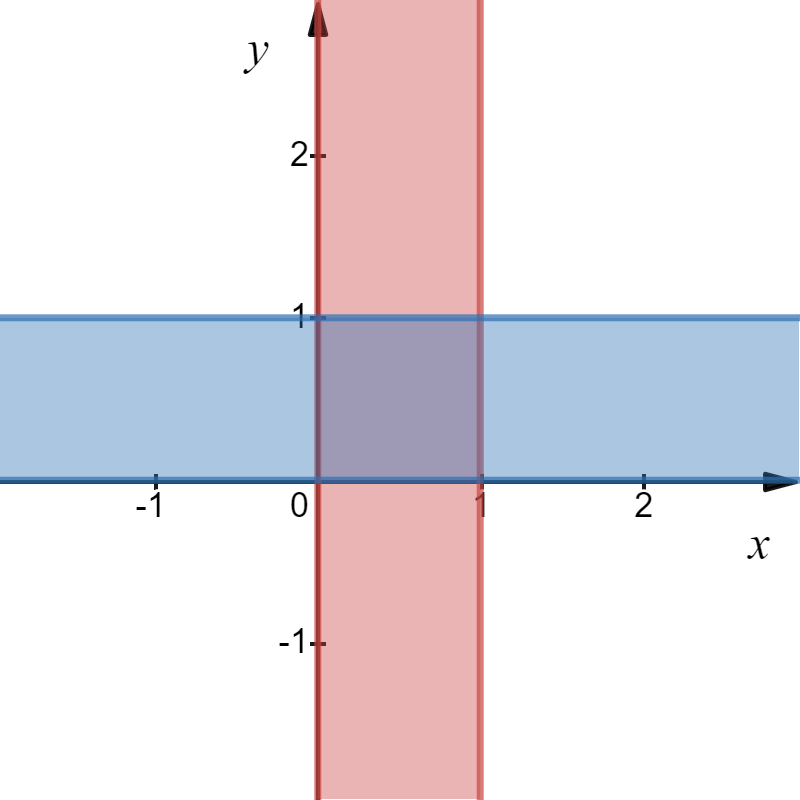
\includegraphics[width=.6\textwidth]{Figures/bounds_1.png}
    \caption{Red band is the set of points $x\in [0,1]$ and the blue band is the set of points $y\in [0,1]$. Where they overlap is the unit square.}
\end{figure}
Yet, we want to create a half triangle of this square subject to the constraint $x\leq y$. Thus, we get the following figure.
\begin{figure}[H]
    \centering
    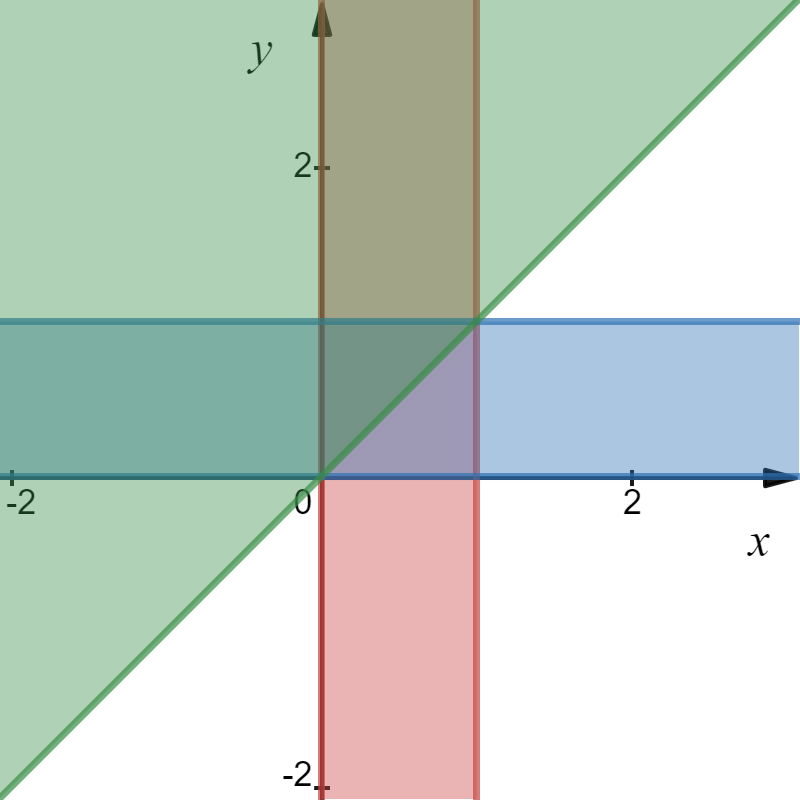
\includegraphics[width=.6\textwidth]{Figures/bounds_2.png}
    \caption{Additional green area is the constraint $x\leq y$.}
\end{figure}
Where every color overlaps is the domain in the $xy$-plane we wish to integrate over. Following the figure and given constraint for intuition, we realize that the bounds for $x$ must depend on $y$. Note, the bounds for $y$ \emph{cannot} depend on $x$ if we integrate $y$ \emph{after} $x$! We can see that the bounds $0\leq x \leq y$ yield the following figure.
\begin{figure}[H]
    \centering
    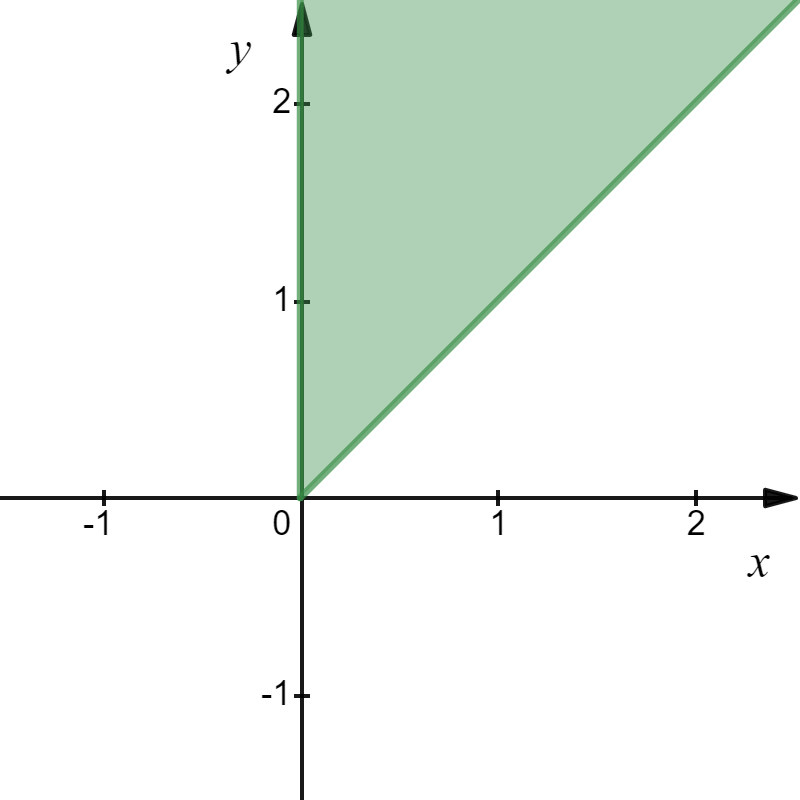
\includegraphics[width=.6\textwidth]{Figures/bounds_3.png}
    \caption{The region where $0\leq x\leq y$.}
\end{figure}
Now, we have determined bounds for $x$ via this analysis and we still need to determine bounds for both $y$ and $z$ (which we have not discussed at all yet!). The bounds for $y$ can be seen by investigating the previous figures. We need $0\leq y \leq 1$ in order to integrate over the half triangle of the unit square -- no more, no less. Hence, we now can put
\[
\iiint_{\Omega} f d\Omega = \int_{z=?}^{z=?} \int_{y=0}^{y=1} \int_{x=0}^{x=y} 2xy +e^{xz} + \sin(y) dxdydz.
\]
Finally, the triangular prism is built by extending this triangle out of the plane in the $z$-direction. Specifically, the prism should go up a height of 4 above the $xy$-plane, and so $z \in [0,4]$. Thus, we now have an integral to compute
\begin{align*}
\iiint_{\Omega} f d\Omega &= \int_{z=0}^{z=4} \int_{y=0}^{y=1} \int_{x=0}^{x=y} 2xy +e^{xz} + \sin(y) dxdydz\\
&= \mathrm{Ei}(4) + \frac{9}{4} - \frac{e^4}{4} - \gamma - \ln(4) + 4\sin(1) -4\cos(1)
&\approx 7.4725,
\end{align*}
where $\mathrm{Ei}$ is the exponential integral (\url{https://en.wikipedia.org/wiki/Exponential_integral}) and $\gamma$ is the Euler--Mascheroni constant (\url{https://en.wikipedia.org/wiki/Euler%27s_constant} which actually relates the harmonic series to the natural log).

This integral was computed using WolframAlpha by inputting:
\begin{verbatim}
integrate[integrate[integrate[2xy+e^(xz)+sin(y),{x,0,y}],{y,0,1}],{z,0,4}]
\end{verbatim}
\end{solution}
\vspace*{1cm}
\textcolor{red}{
\noindent \textbf{Rubric:}
\begin{enumerate}[(a)]
    \item \textbf{(1 pt.)} Correct bounds for $x$ integral. \textbf{(1 pt.)} Correct bounds for $y$ and $z$ parts of integral. \textbf{(1 pt.)} Correct value of the integral.
\end{enumerate}
}

\end{document}